% siminos/presentations/kittens/why.tex        pdflatex why; biber why
% $Author: predrag $ $Date: 2021-12-07 18:54:06 -0500 (Tue, 07 Dec 2021) $

% remember to update \date{December 6, 2021}

% when you get      LaTeX Error: Command \block already defined.
%                   l.512 \newcommand{\block}[1]{\ensuremath{#1}}
% press [Enter] once

% kittens.tex FROZEN, split into                            2020-09-25
%    why.tex
%    Bernoulli.tex   Bernoulli.mp4
%    templatt.tex    templatt.mp4
%    catlatt.tex     catlatt.mp4
%    timeDead.tex

%  lectures/QFT20/ kittens.pdf saved as                     2020-09-27
%          ChaosBook.org/overheads/spatiotemporal/QFT20.pdf
%  started with siminos/presentations/GTmath18/GTmath18.tex 2018-03-02
%  started with siminos/presentations/KITP17/UCSB17.tex     2017-01-26
%  started with siminos/presentations/Israel16/Israel16.tex 2016-08-17
%  started with siminos/presentations/GTmap16/GTmap16.tex   2016-08-17
%  started with talks/predrag/NBI16/NBI16.tex               2016-04-25
%  started with talks/predrag/RoySoc16/RoySoc16.tex         2016-04-25

                        \newif\ifboyscout\boyscouttrue          %% comments     %%
                        \newif\ifsubmission\submissionfalse     %% internal     %%
                        \newif\ifblog\blogfalse %% section shared with blogCats %%

\input ../../inputs/layoutBeamer
\usepackage[font=scriptsize, labelfont=bf]{caption}
\usepackage[
    backend=biber,  %bibtex,
    sorting=nyt,
    %refsection=chapter,
    %citereset=chapter,
    style=numeric, %alphabetic, % %style=authoryear,
    natbib=true,
    style=phys, % aps
    biblabel= brackets, % superscript, %
    articletitle=false, % true,  % false, % aps
    %chaptertitle=true,  % aip;  % false, % aps
    pageranges = true , % aip: the full range
             % = false, % aps: only the first page being printed
    sortlocale=en_US,
    firstinits=true,
    url=false, %true,  %
    doi=false, %true,
    eprint=false
]{biblatex}
\addbibresource{../../bibtex/siminos.bib}
\setbeamerfont{footnote}{size=\tiny}
%\input ../../inputs/def % no edits, always from dasbuch/book/inputs
\input defsKittens
\input ../../inputs/defsBeamer
\renewcommand{\Ssym}[1]{{\ensuremath{m_{#1}}}}    % Boris
% \newcommand{\Ssym}[1]{{\ensuremath{s_{#1}}}}  % ChaosBook
% \newcommand{\D}{\mathcal{D}}
% \newcommand{\gd}{\mathsf{g}}

\begin{document}
\title{
{\huge herding cats} %\catlatt}
    \\
{a chaotic field theory}
}
\author{P. Cvitanovi\'c}
\author[Cvitanovi\'c]
{
  \textcolor{green!50!black}{
  {Predrag~Cvitanovi\'c
   and
   Han Liang
%   \\
%  Matt Gudorf,
  }	%\inst{1}
  }
}
\institute
{
               Georgia Tech
 \\
%  \inst{1}%
%\HREF{https://itsatcuny.org/calendar/chaos-and-quantum-field-theory}
%{ITS Symposium on Chaos and Quantum Field Theory}
    {\scriptsize
\HREF{https://ChaosBook.org/overheads/spatiotemporal}
 {ChaosBook.org/overheads/spatiotemporal}
 \\ $\to$ Chaotic field theory slides
    }
 }
\date{November 17, 2021}

%%%%%%%%%%%%%%%%%%%%%%%%%%%%%%%%%%%%%%%%%%%%%%%%%%%%%%%%%%%%%%%%%%%%%%%%
\begin{frame}{} %herding cats}
\begin{center}
\hfill
\includegraphics[width=0.95\textheight]{DawnBishopCats}
\end{center}
\end{frame} %%%%%%%%%%%%%%%%%%%%%%%%%%%%%%%%%%%%%%%%%%%%%%

\begin{frame}
  \titlepage
\end{frame} %%%%%%%%%%%%%%%%%%%%%%%%%%%%%%%%%%%%%%%%%%%%%%


%\section[what this talk is about]
% {what this talk is about}
%
%%%%%%%%%%%%%%%%%%%%%%%%%%%%%%%%%%%%%%%%%%%%%%%%%%%%%%%%%%
\begin{frame}{overview}
\begin{enumerate}
              \item {\Large
what is this about
                  }\textcolor{gray}{\small
%\\{\scriptsize \em
%  (to skip the motivational blah blah: go to part \textcolor{red}{\ref{spacetimeFT}})
%  }
              \item
chaos - a short course
              \item
\templatt
              \item
\catlatt
              \item
chaotic field theory
              \item
space is time
              \item
bye bye, dynamics
                    }
            \end{enumerate}
\end{frame} %%%%%%%%%%%%%%%%%%%%%%%%%%%%%%%%%%%%%%%%%%%%%%

%%%%%%%%%%%%%%%%%%%%%%%%%%%%%%%%%%%%%%%%%%%%%%%%%%%%%%%%%%%%%%%%%%%%%%%%
\begin{frame}{Q. what is a chaotic field theory?}
    \begin{block}{A. it is a field theory}
\textcolor{blue}{field configuration} \Xx\ probability
\[
p(\Xx)\,=\, \frac{1}{Z}\,e^{-S[\Xx]}
\,,\qquad Z=Z[0]
\] % ee{ProbConf}
\textcolor{blue}{partition function} $=$ sum over configurations
\beq
Z[\source]	% = e^{W[\source]}
    \,=\, \int [d\ssp]\,e^{-S[\Xx] + \Xx \cdot \source}
    \,,\qquad
\left[ d\ssp\right] = \prod_{z}^{\lattice} \frac{d\ssp_z}{\sqrt{2 \pi}}
\label{n-pt-corr}
\eeq
    \end{block}
%\textcolor{blue}{`source'} $\source$
\bigskip

    \begin{block}{example : Euclidean {$\phi^4$} theory \textcolor{blue}{action}}
\bea
S[\Xx] &=& \int dx^d \left\{ \frac{1}{2} \sum_{i =1}^d
(\partial_{\mu}\ssp(x))^2 + \frac{\mu^2}{2}\ssp(x)^2 + \frac{g}{4!}\ssp(x)^4
\right\}
\eea
    \end{block}
\end{frame} %%%%%%%%%%%%%%%%%%%%%%%%%%%%%%%%%%%%%%%%%%%%%%

%%%%%%%%%%%%%%%%%%%%%%%%%%%%%%%%%%%%%%%%%%%%%%%%%%%%%%%%%%
\begin{frame}{Q. why a "chaotic" field theory?}
\vfill
\begin{center}
{\huge turbulence !}
\end{center}
\vfill
\end{frame} %%%%%%%%%%%%%%%%%%%%%%%%%%%%%%%%%%%%%%%%%%%%%%

%%%%%%%%%%%%%%%%%%%%%%%%%%%%%%%%%%%%%%%%%%%%%%%%%%%%%%%%%%
\begin{frame}{a motivation : need a theory of {\Huge large} turbulent domains}
pipe flow close to onset of turbulence
\footnote{M.~Avila and B.~Hof, {Phys. Rev. \bf E 87} (2013)}
\begin{center}
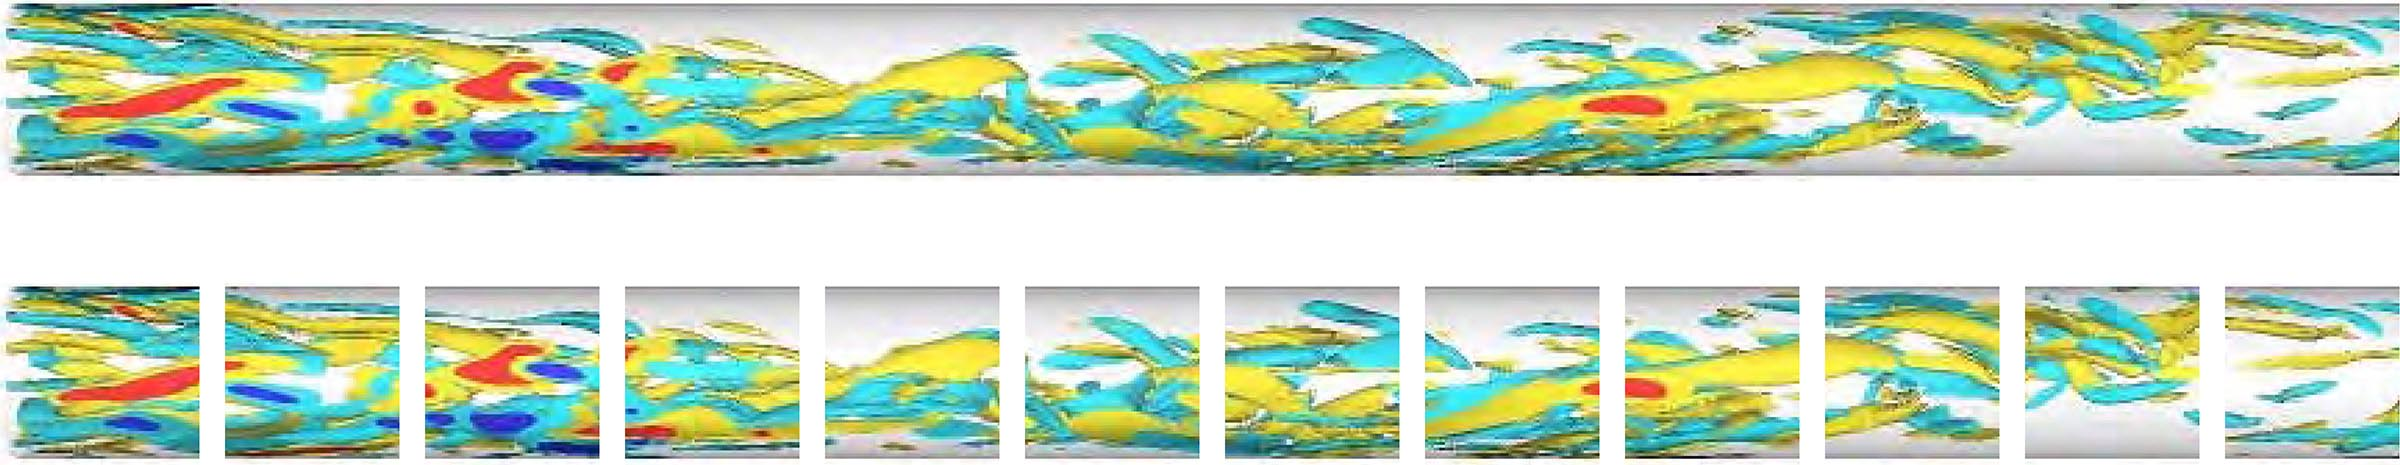
\includegraphics[width=1.0\textwidth]{AviHof13fig4CLM}
\end{center}
we have a detailed theory of {\small \textcolor{blue}{small}} turbulent fluid cells

\bigskip

can we can we construct the \textcolor{red}{infinite} pipe by coupling small turbulent cells ?
\bigskip

\textcolor{blue}{what would that theory look like ?}
\end{frame} %%%%%%%%%%%%%%%%%%%%%%%%%%%%%%%%%%%%%%%%%%%%%%

%%%%%%%%%%%%%%%%%%%%%%%%%%%%%%%%%%%%%%%%%%%%%%%%%%%%%%%%%%
\begin{frame}{the goal}
\vfill

\begin{center}
{\Large build
\\
a \textcolor{blue}{chaotic field theory}
\medskip

from
\\
the simplest \textcolor{blue}{chaotic blocks}
}
\end{center}

\vfill
using
\begin{itemize}
  \item
\textcolor{blue}{time invariance}
  \item
\textcolor{blue}{space invariance}
\end{itemize}
 of the defining partial differential equations
\end{frame} %%%%%%%%%%%%%%%%%%%%%%%%%%%%%%%%%%%%%%%%%%%%%%

%%%%%%%%%%%%%%%%%%%%%%%%%%%%%%%%%%%%%%%%%%%%%%%%%%%%%%%%%%
\begin{frame}{Dreams of Grand Schemes : solve}
 \begin{center}
   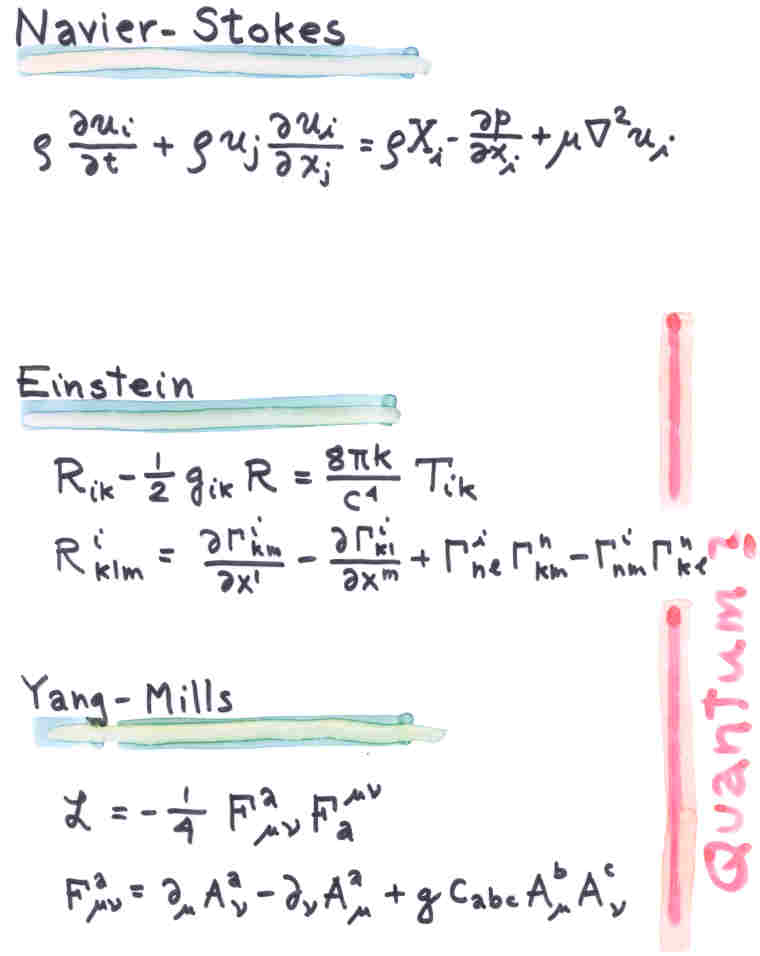
\includegraphics[width=0.60\textwidth]{02-DreamEqs}
 \end{center}
\end{frame}

%%%%%%%%%%%%%%%%%%%%%%%%%%%%%%%%%%%%%%%%%%%%%%%%%%%%%%%%%%
\begin{frame}{QFT path integrals : semi-classical WKB quantization}
  \begin{columns}
  \column{0.42\textwidth}
\begin{block}{a local unstable extremum}
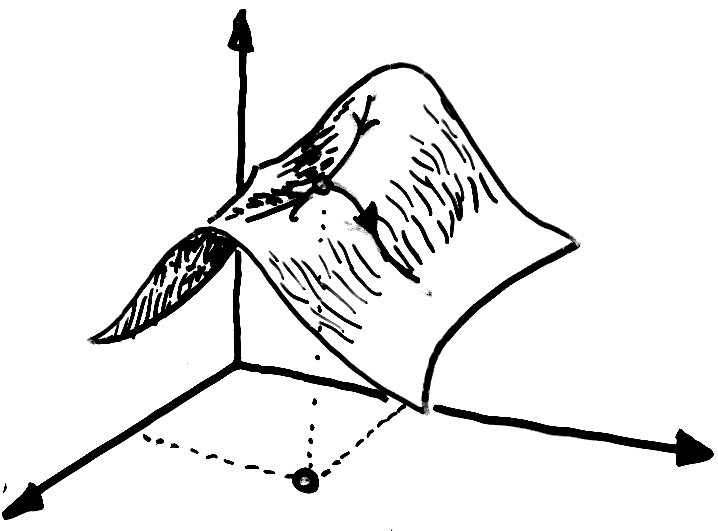
\includegraphics[width=1.00\textwidth,clip=true]{saddle}%
\end{block}
  \column{0.50\textwidth}
\begin{block}{a fractal set of saddles}
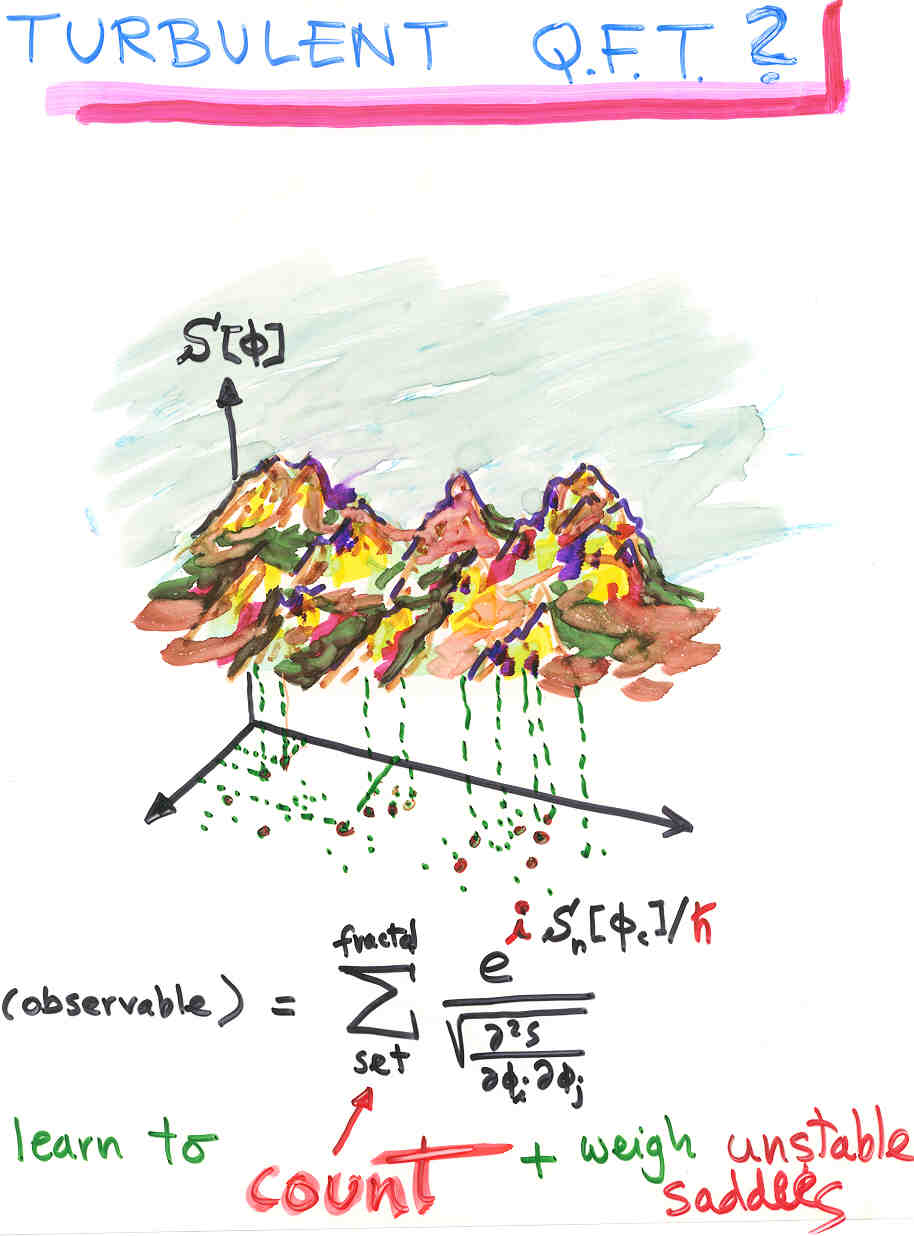
\includegraphics[width=1.00\textwidth,clip=true]{pde2}%
\end{block}
  \end{columns}
\end{frame} %%%%%%%%%%%%%%%%%%%%%%%%%%%%%%%%%%%%%%%%%%%%%%

%%%%%%%%%%%%%%%%%%%%%%%%%%%%%%%%%%%%%%%%%%%%%%%%%%%%%%%%%%
\begin{frame}{take-home :   }
\begin{center}
            \begin{minipage}[c]{0.40\textwidth}\begin{center}
{\color{purple}harmonic} field theory
\bigskip

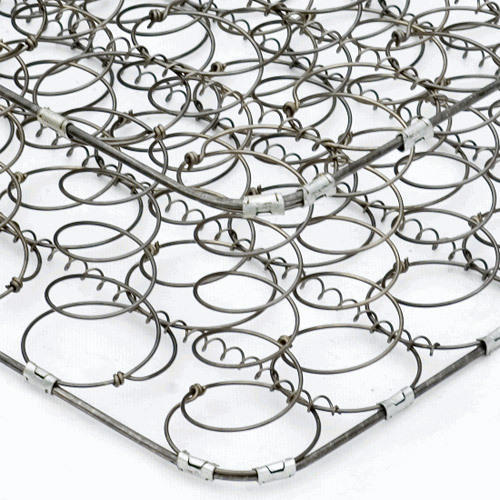
\includegraphics[width=0.85\textwidth]{mattressSpring}\\
{\color{blue}tight-binding} model \\ ({\color{blue}Helmholtz})
            \end{center}\end{minipage}
            \hspace{2ex}
            \begin{minipage}[c]{0.46\textwidth}\begin{center}
{\color{purple}chaotic} field theory\\
\bigskip
\bigskip
\bigskip

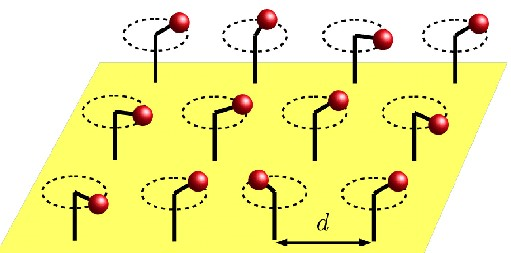
\includegraphics[width=1.0\textwidth]{flagellum1}\\
\bigskip

Euclidean {\color{blue}Klein-Gordon} \\ (damped {\color{blue}Poisson})
            \end{center}\end{minipage}
\end{center}
\end{frame} %%%%%%%%%%%%%%%%%%%%%%%%%%%%%%%%%%%%%%%%%%%%%%

%%%%%%%%%%%%%%%%%%%%%%%%%%%%%%%%%%%%%%%%%%%%%%%%%%%%%%%%%%
\begin{frame}{take-home :   }
\begin{center}
            \begin{minipage}[c]{0.40\textwidth}\begin{center}
{\color{purple}harmonic} field theory
\bigskip

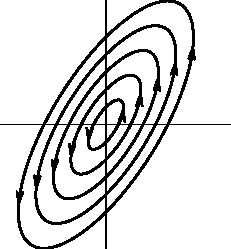
\includegraphics[width=0.35\textheight]{twodlinearEll}\\
\bigskip

{\color{blue}oscillatory eigenmodes}
            \end{center}\end{minipage}
            \hspace{2ex}
            \begin{minipage}[c]{0.46\textwidth}\begin{center}
{\color{purple}chaotic} field theory\\
\bigskip

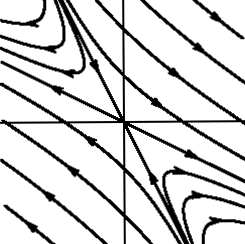
\includegraphics[width=0.35\textheight]{twodlinearHyp}\\
\bigskip

{\color{blue}hyperbolic instabilities}
            \end{center}\end{minipage}
\end{center}
\end{frame} %%%%%%%%%%%%%%%%%%%%%%%%%%%%%%%%%%%%%%%%%%%%%%

%%%%%%%%%%%%%%%%%%%%%%%%%%%%%%%%%%%%%%%%%%%%%%%%%%%%%%%%%%
\begin{frame}{the very short answer : POT}
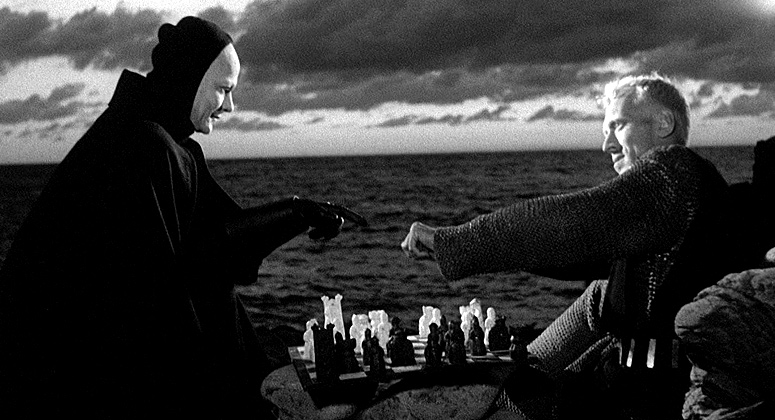
\includegraphics[width=1.0\textwidth]{MvSydow7seal.jpg}
\bigskip
if you win : I teach you how

\vfill\hfill (for details, see \wwwcb{})
\end{frame}  %%%%%%%%%%%%%%%%%%%%%%%%%%%%%%%%%%%%%%%%%%%%%

\section[a coin toss]
 {a coin toss}

%%%%%%%%%%%%%%%%%%%%%%%%%%%%%%%%%%%%%%%%%%%%%%%%%%%%%%%%%%
\begin{frame}{}
\begin{bartlett}{
Mephistopheles knocks at Faust's door and says, ``Du
mu{\ss}t es dreimal sagen!"
\\{\color{yellow}.}\qquad
{\scriptsize\emph{``You have to say it three times"}}
        }
\bauthor{
Johann Wolfgang von Goethe
\\{\color{yellow}.}\qquad\quad
{\em Faust I - Studierzimmer 2.~Teil}%\rf{GoetheIstuZim1806}
    }
\end{bartlett}
\vfill
\begin{enumerate}
              \item \textcolor{gray}{\small
what this is about
                  }
              \item {\Large
\HREF{http://ChaosBook.org/overheads/spatiotemporal/Bernoulli.pdf}
{coin toss}
                  }\textcolor{gray}{\small
              \item
\HREF{http://ChaosBook.org/overheads/spatiotemporal/templatt.pdf}
{\templatt}
              \item
\HREF{http://ChaosBook.org/overheads/spatiotemporal/catlatt.pdf}
{\catlatt}
              \item
\HREF{http://ChaosBook.org/overheads/spatiotemporal/timeDead.pdf}
{bye bye, dynamics}
                    }
            \end{enumerate}
\end{frame} %%%%%%%%%%%%%%%%%%%%%%%%%%%%%%%%%%%%%%%%%%%%%%

\end{document}
